% F087｜steps 原创简明教学示意图
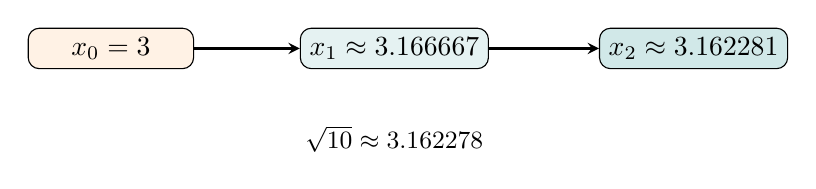
\begin{tikzpicture}[>=stealth,node distance=1cm]
\node[draw,rounded corners,fill=orange!10,minimum width=2.1cm] (a) at (0,0) {$x_0=3$};
\node[draw,rounded corners,fill=teal!10,minimum width=2.3cm] (b) at (3.6,0) {$x_1\approx3.166667$};
\node[draw,rounded corners,fill=teal!18,minimum width=2.3cm] (c) at (7.4,0) {$x_2\approx3.162281$};
\draw[->,thick] (a)--(b);\draw[->,thick] (b)--(c);
\node at (3.6,-1.15) {\small $\sqrt{10}\approx3.162278$};
\end{tikzpicture}
